\documentclass[10pt,a4paper]{article}
\usepackage[T1]{fontenc}\usepackage[utf8]{inputenc}
\usepackage{helvet,graphicx,tikz,amsmath}
\usepackage[a4paper,margin=0pt]{geometry}
\renewcommand{\familydefault}{\sfdefault}\pagestyle{empty}
\pdfinfoomitdate=1\pdftrailerid{}
\definecolor{muted}{HTML}{747474}
\definecolor{rule}{HTML}{D9D9D9}
% Native-scale selection sheets.
\begin{document}
\null\begin{tikzpicture}[remember picture,overlay,x=1cm,y=-1cm]
\begin{scope}[shift={(current page.north west)}]
\node[anchor=north west,inner sep=0,font=\bfseries\fontsize{15}{18}\selectfont] at (1.6,.85) {B / Wie viel Vergangenheit fehlt?};
\node[anchor=north west,inner sep=0,font=\fontsize{10}{12}\selectfont,text=muted] at (1.6,1.60) {Wähle eine B- und eine C-Variante. Die Nummern müssen nicht übereinstimmen.};
\node[anchor=north west,inner sep=0,font=\bfseries\fontsize{10.5}{12}\selectfont] at (1.60,2.30) {B1  /  Mögliche Ausgaben werden enger};
\node[anchor=north west,inner sep=0] at (1.60,2.78) {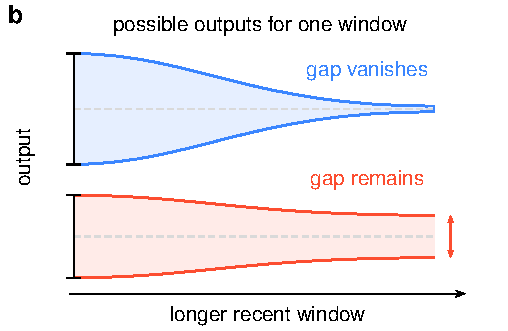
\includegraphics[width=8.60cm]{b1.pdf}};
\node[anchor=north west,inner sep=0,text width=8.60cm,align=left,font=\fontsize{10}{12}\selectfont] at (1.60,8.65) {Mehr Kontext kann die Ausgabeunsicherheit beliebig verkleinern oder einen bleibenden Rest lassen.};
\node[anchor=north west,inner sep=0,font=\bfseries\fontsize{10.5}{12}\selectfont] at (10.80,2.30) {B2  /  Gleiches Fenster, verschiedene Vergangenheit};
\node[anchor=north west,inner sep=0] at (10.80,2.78) {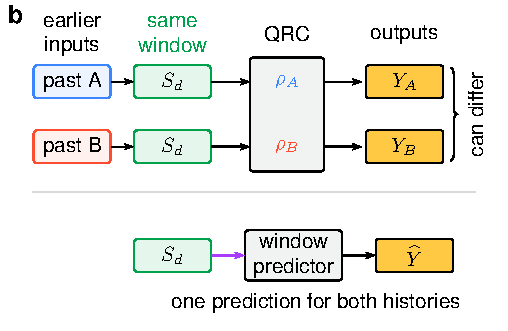
\includegraphics[width=8.60cm]{b2.pdf}};
\node[anchor=north west,inner sep=0,text width=8.60cm,align=left,font=\fontsize{10}{12}\selectfont] at (10.80,8.65) {Gleiches Fenster, zwei mögliche QRC-Ausgaben: Ein Fenstermodell muss für beide dieselbe Vorhersage machen.};
\node[anchor=north west,inner sep=0,font=\bfseries\fontsize{10.5}{12}\selectfont] at (1.60,10.30) {B3  /  Schrittweise weniger Mehrdeutigkeit};
\node[anchor=north west,inner sep=0] at (1.60,10.78) {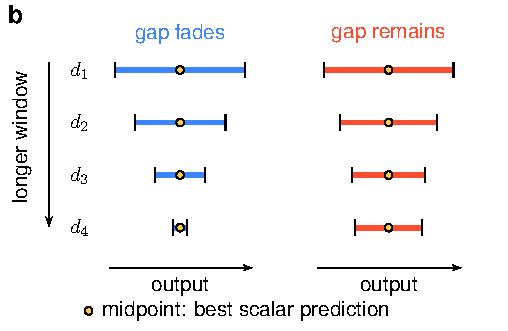
\includegraphics[width=8.60cm]{b3.pdf}};
\node[anchor=north west,inner sep=0,text width=8.60cm,align=left,font=\fontsize{10}{12}\selectfont] at (1.60,16.65) {Die Balken umspannen mögliche Ausgaben; ihr Mittelpunkt minimiert den größten skalaren Vorhersagefehler.};
\node[anchor=north west,inner sep=0,font=\bfseries\fontsize{10.5}{12}\selectfont] at (10.80,10.30) {B4  /  Kontext bis zur Fehlertoleranz};
\node[anchor=north west,inner sep=0] at (10.80,10.78) {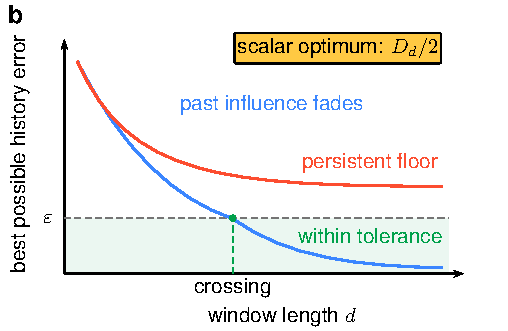
\includegraphics[width=8.60cm]{b4.pdf}};
\node[anchor=north west,inner sep=0,text width=8.60cm,align=left,font=\fontsize{10}{12}\selectfont] at (10.80,16.65) {Genügend Kontext kann den Geschichtsfehler unter die Toleranz bringen. Ein bleibender Rest kann dies verhindern.};
\node[anchor=north west,inner sep=0,font=\bfseries\fontsize{10.5}{12}\selectfont] at (1.60,18.30) {B5  /  Was von früher übrig bleibt};
\node[anchor=north west,inner sep=0] at (1.60,18.78) {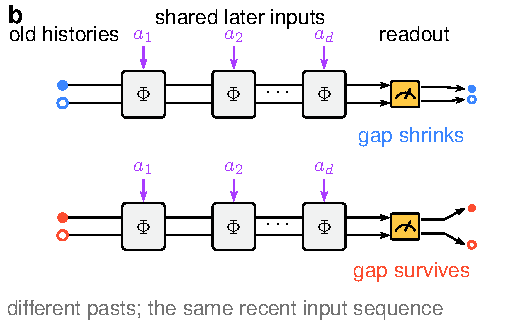
\includegraphics[width=8.60cm]{b5.pdf}};
\node[anchor=north west,inner sep=0,text width=8.60cm,align=left,font=\fontsize{10}{12}\selectfont] at (1.60,24.65) {Gleiche spätere Eingaben: Ein alter Unterschied wird abgeschwächt oder bleibt in der Ausgabe sichtbar.};
\draw[rule] (10.8,19.0)--(19.4,19.0);
\node[anchor=north west,inner sep=0,text width=8.60cm,align=left,font=\fontsize{11}{14}\selectfont] at (10.8,19.4) {Alle Varianten erklären die Grenze durch fehlende Vergangenheit. Ein kleines Geschichtsproblem allein garantiert noch keine ausreichend leistungsfähige konkrete QELM.};
\node[anchor=north west,inner sep=0,text width=8.60cm,align=left,font=\fontsize{10}{12}\selectfont,text=muted] at (10.8,22.2) {Alle Zeichnungen sind konzeptionelle Erklärungen, keine neuen Messdaten. Das aktuelle Paper bleibt bis zur Auswahl unverändert.};
\draw[rule] (1.6,27.0)--(19.4,27.0);
\node[anchor=north west,inner sep=0,text width=17.8cm,align=left,font=\fontsize{9}{11}\selectfont,text=muted] at (1.6,27.3) {Originalgröße je Entwurf: 8,6 $\times$ 5,6 cm; 10-pt-Beschriftung. Gestalterische Referenz: Fig. 1 in Freiheit und Campaioli, \textit{Superextensive learning in quantum reservoirs at the onset of information scrambling}. Die Diagramme hier erklären ausschließlich den Inhalt unseres Papers.};
\end{scope}\end{tikzpicture}
\newpage
\null\begin{tikzpicture}[remember picture,overlay,x=1cm,y=-1cm]
\begin{scope}[shift={(current page.north west)}]
\node[anchor=north west,inner sep=0,font=\bfseries\fontsize{15}{18}\selectfont] at (1.6,.85) {C / Welche Zustandsunterschiede zählen?};
\node[anchor=north west,inner sep=0,font=\fontsize{10}{12}\selectfont,text=muted] at (1.6,1.60) {Wähle eine B- und eine C-Variante. Die Nummern müssen nicht übereinstimmen.};
\node[anchor=north west,inner sep=0,font=\bfseries\fontsize{10.5}{12}\selectfont] at (1.60,2.30) {C1  /  Zwei Zustände, gleiche Messung};
\node[anchor=north west,inner sep=0] at (1.60,2.78) {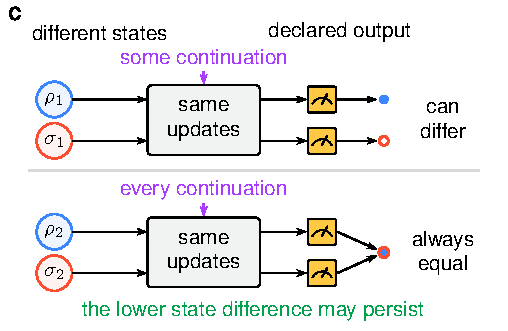
\includegraphics[width=8.60cm]{c1.pdf}};
\node[anchor=north west,inner sep=0,text width=8.60cm,align=left,font=\fontsize{10}{12}\selectfont] at (1.60,8.65) {Verschiedene Zustände können unterscheidbare Ausgaben liefern - oder unter jeder Fortsetzung identische Ausgaben.};
\node[anchor=north west,inner sep=0,font=\bfseries\fontsize{10.5}{12}\selectfont] at (10.80,2.30) {C2  /  Erreicht der Unterschied den Ausgang?};
\node[anchor=north west,inner sep=0] at (10.80,2.78) {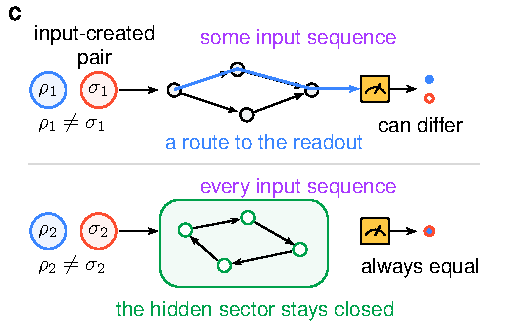
\includegraphics[width=8.60cm]{c2.pdf}};
\node[anchor=north west,inner sep=0,text width=8.60cm,align=left,font=\fontsize{10}{12}\selectfont] at (10.80,8.65) {Ein Unterschied zählt, wenn er die Ausgabe erreichen kann. Ein dauerhaft unsichtbarer Bereich zählt nicht.};
\node[anchor=north west,inner sep=0,font=\bfseries\fontsize{10.5}{12}\selectfont] at (1.60,10.30) {C3  /  Heute gleich, später unterscheidbar};
\node[anchor=north west,inner sep=0] at (1.60,10.78) {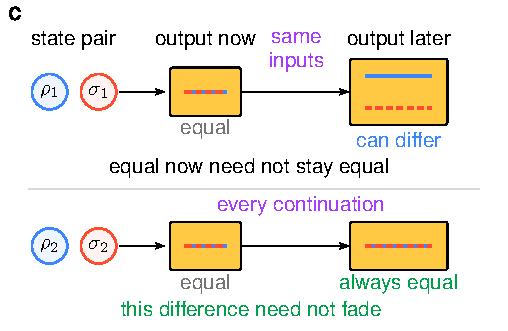
\includegraphics[width=8.60cm]{c3.pdf}};
\node[anchor=north west,inner sep=0,text width=8.60cm,align=left,font=\fontsize{10}{12}\selectfont] at (1.60,16.65) {Gleiche Ausgaben jetzt können später auseinandergehen. Nur Gleichheit unter jeder Fortsetzung macht den Unterschied irrelevant.};
\node[anchor=north west,inner sep=0,font=\bfseries\fontsize{10.5}{12}\selectfont] at (10.80,10.30) {C4  /  Ein dauerhaft unsichtbarer Unterschied};
\node[anchor=north west,inner sep=0] at (10.80,10.78) {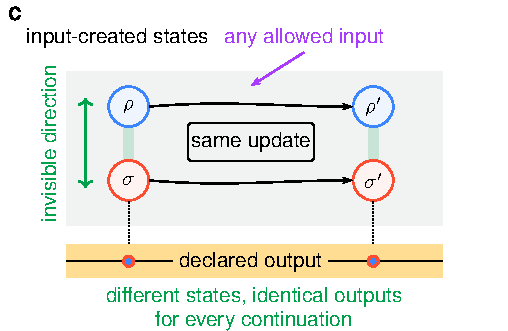
\includegraphics[width=8.60cm]{c4.pdf}};
\node[anchor=north west,inner sep=0,text width=8.60cm,align=left,font=\fontsize{10}{12}\selectfont] at (10.80,16.65) {Bleibt eine Zustandsdifferenz unter allen Eingaben unsichtbar, müssen die internen Zustände nicht zusammenfallen.};
\node[anchor=north west,inner sep=0,font=\bfseries\fontsize{10.5}{12}\selectfont] at (1.60,18.30) {C5  /  Gleiches Verhalten, verschiedene Zustände};
\node[anchor=north west,inner sep=0] at (1.60,18.78) {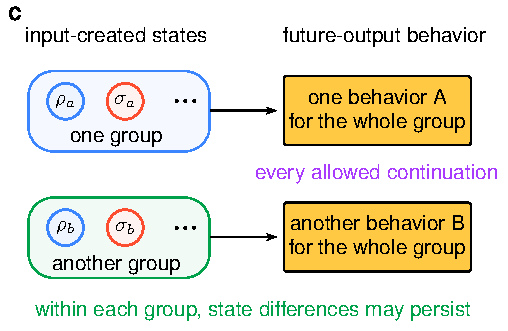
\includegraphics[width=8.60cm]{c5.pdf}};
\node[anchor=north west,inner sep=0,text width=8.60cm,align=left,font=\fontsize{10}{12}\selectfont] at (1.60,24.65) {Verschiedene Zustände gehören zusammen, wenn sie für jede gemeinsame Fortsetzung dieselben Ausgaben erzeugen.};
\draw[rule] (10.8,19.0)--(19.4,19.0);
\node[anchor=north west,inner sep=0,text width=8.60cm,align=left,font=\fontsize{11}{14}\selectfont] at (10.8,19.4) {Gleiche Ausgabe jetzt genügt nicht. Unsichtbar bedeutet hier: keine erlaubte gemeinsame Fortsetzung kann den Unterschied in den festgelegten Ausgaben sichtbar machen.};
\node[anchor=north west,inner sep=0,text width=8.60cm,align=left,font=\fontsize{10}{12}\selectfont,text=muted] at (10.8,22.2) {Alle Zeichnungen sind konzeptionelle Erklärungen, keine neuen Messdaten. Das aktuelle Paper bleibt bis zur Auswahl unverändert.};
\draw[rule] (1.6,27.0)--(19.4,27.0);
\node[anchor=north west,inner sep=0,text width=17.8cm,align=left,font=\fontsize{9}{11}\selectfont,text=muted] at (1.6,27.3) {Originalgröße je Entwurf: 8,6 $\times$ 5,6 cm; 10-pt-Beschriftung. Gestalterische Referenz: Fig. 1 in Freiheit und Campaioli, \textit{Superextensive learning in quantum reservoirs at the onset of information scrambling}. Die Diagramme hier erklären ausschließlich den Inhalt unseres Papers.};
\end{scope}\end{tikzpicture}
\end{document}
